\documentclass[aspectratio=169]{beamer}
\usetheme{hogent}
\usecolortheme{hgwhite} % witte achtergrond, zwarte tekst

%% common.tex -- Code die in elk .tex-bestand terug komt

%% Packages

\usepackage[dutch]{babel}
\usepackage{graphicx}
\usepackage{comment,enumerate,hyperref}
\usepackage{amsmath,amsfonts,amssymb}
\usepackage{eurosym}
\usepackage{booktabs}
\usepackage{multicol,multirow}
\usepackage{listings}

\usepackage[outputdir=out]{minted}
%\usepackage{minted}

\usepackage[backend=biber,style=apa]{biblatex}
\DeclareLanguageMapping{dutch}{dutch-apa}

\usepackage{csquotes}

%% Variabelen, elk academiejaar aan te passen
\newcommand{\academicyear}{2023--2024 (revisie: \today)}
\newcommand{\lecturers}{Thomas Aelbrecht \and Thomas Parmentier \and Bert Van Vreckem}
\newcommand{\coursename}{Research Methods (IT)}

%% Macro's en commando's

%% \alertbox: een kader voor tekst die moet opvallen
\newcommand{\alertbox}[2][hgblue]{%
  \setbeamercolor{alertbox}{bg=#1,fg=white}
  \begin{beamercolorbox}[sep=2pt,center]{alertbox}
    \textbf{#2}
  \end{beamercolorbox}
}

\addbibresource{rm4-bibliografie.bib}

%---------- Info over de presentatie ------------------------------------------

\title{Module 4. Een bibliografische databank bijhouden.}
\subtitle{Research Methods}
\author{\lecturers}   % Pas waarden aan in common.tex
\date{\academicyear}

\begin{document}

\begin{frame}
  \maketitle
\end{frame}

\begin{frame}
  \frametitle{Inhoud}

  \tableofcontents
\end{frame}

\section{Literatuurstudie in {\LaTeX}.}

\begin{frame}
  \frametitle{Bibliografische databank}

  \begin{itemize}
    \item = Software om bronnen gestructureerd bij te houden
    \item Fulltext + metadata
    \item Genereren correct opgemaakte literatuurlijst
    \item Syn.: reference management software
  \end{itemize}

\end{frame}

\begin{frame}
  \frametitle{Voorbeelden}

  \begin{itemize}
    \item Endnote: commercieel
    \item Mendeley: commercieel, gratis
    \item JabRef: open source
  \end{itemize}

\end{frame}

\begin{frame}[plain]
  \frametitle{JabRef}

  \centering
  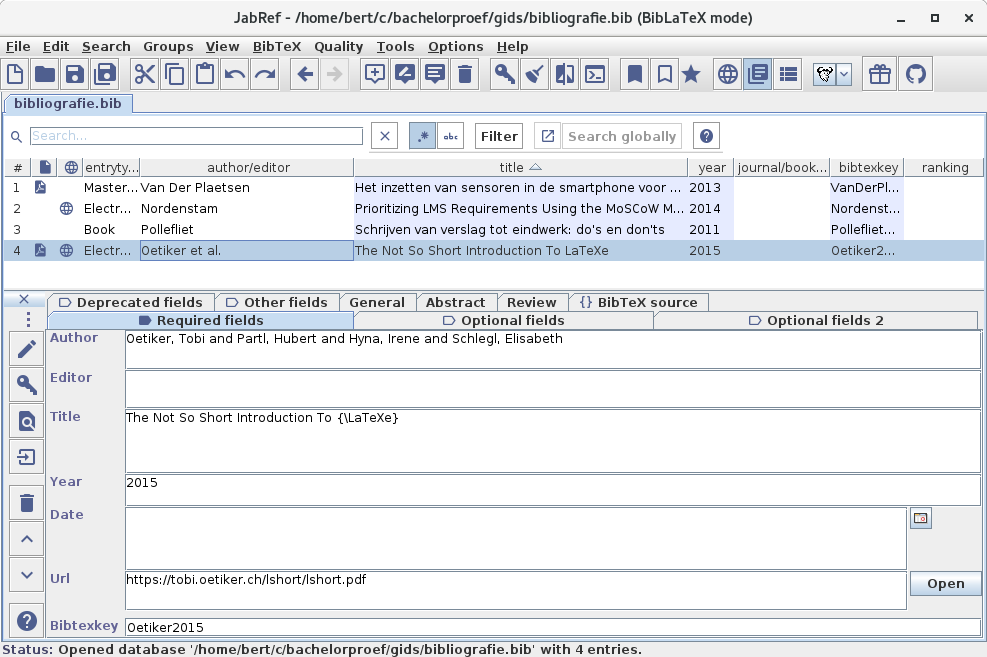
\includegraphics[height=.8\textheight]{4/jabref-screenshot}

\end{frame}

\begin{frame}
  \frametitle{JabRef instellingen}

  Options > Preferences

  \begin{itemize}
    \item General
    \begin{itemize}
      \item Default encoding: \textbf{UTF-8}
      \item Default library mode: \textbf{biblatex}
    \end{itemize}
    \item Linked files
    \begin{itemize}
      \item Main file directory: (pad naar map waar je PDF's bijhoudt)
    \end{itemize}
  \item Entry Preview: APA 7th edition
  \end{itemize}

\end{frame}

\begin{frame}[fragile]
  \frametitle{Bronvermelding en referentielijst in {\LaTeX}.}

  Bib{\LaTeX} en Biber

  \bigskip

  \verb|artikel.tex|: Hoofdtekst\\
  \verb|artikel.bib|: Bibliografische databank (bewerk met bv.~JabRef)

  \bigskip

  Preamble:

  \begin{verbatim}
  \usepackage[backend=biber,style=apa]{biblatex}
  \DeclareLanguageMapping{dutch}{dutch-apa}
  \addbibresource{artikel.bib}
  \end{verbatim}

  \textbf{Opm.}\ Reeds voorzien in het sjabloon!

\end{frame}

\section{Een bibliografische databank aanleggen.}

\begin{frame}
  \frametitle{Bibliografische gegevens in Jabref.}

  Info die \textbf{altijd} ingevuld moet worden:

  \begin{description}
    \item[Author] Persoon/Organisatie opgegeven als auteur
    \item[Title] v/h artikel, boek, \ldots
    \item[Date] (of Year): datum van publicatie (\texttt{jjjj-mm-dd})
    \item[Bibtexkey] id van deze bron, gebruikt bij refereren (tip: klik op sleutel-icoon)
  \end{description}

  \bigskip

  Kan je één van deze velden niet invullen? Dan is wellicht geen geschikte bron!
\end{frame}

\begin{frame}
  \frametitle{Het auteursveld}

  Gebruik altijd dit formaat:

  \begin{itemize}
    \item Personen: ``Familienaam, Voornaam and Familienaam, Voornaam and Familienaam, Voornaam\ldots''
    \item Organisatie: tussen accolades bv.\ ``\{The Linux Foundation\}''
  \end{itemize}

\end{frame}

\begin{frame}[fragile,plain]
  \frametitle{Bibliografische gegevens in Jabref.}
  \framesubtitle{Extra info voor Article}

  \begin{description}
    \item[Journal] Naam van het tijdschrift
    \item[Volume] Jaargang
    \item[Number] Nummer binnen de jaargang (optioneel)
    \item[Pages] \verb|mmm--nnn|
  \end{description}

  \bigskip

  \textbf{Voorbeeld:}

  \fullcitebib{Anscombe1973}
\end{frame}

\begin{frame}
  \frametitle{Tip: velden automatisch invullen}

  \begin{itemize}
    \item Elsevier, Springer, \ldots\ hebben Bib\LaTeX{} exportfunctie
    \item Plakken in tabblad ``BibTeX source''
  \end{itemize}

  \bigskip

  \centering
  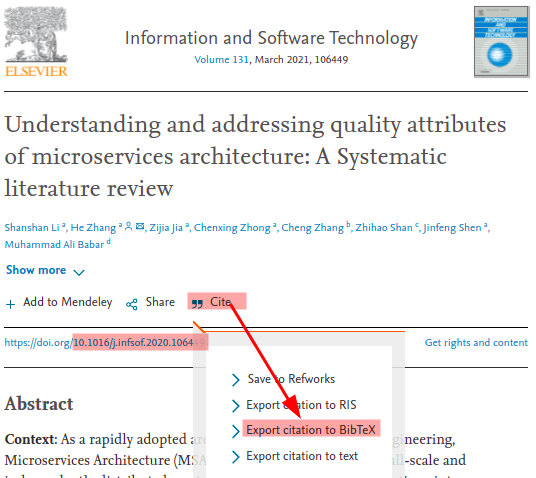
\includegraphics[height=.6\textheight]{4/elsevier-cite-doi}

\end{frame}

\begin{frame}
  \frametitle{Tip: velden automatisch invullen}

  \begin{itemize}
    \item DOI = Digital Object Identifier
    \item Unieke code voor een publicatie
    \item Jabref: General > DOI > Get Bibtex data from DOI
  \end{itemize}

  \bigskip

  \centering
  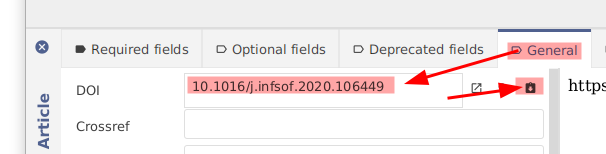
\includegraphics[height=.3\textheight]{4/jabref-doi}

\end{frame}

\begin{frame}[plain]
  \frametitle{Tip: velden automatisch invullen}

  \centering
  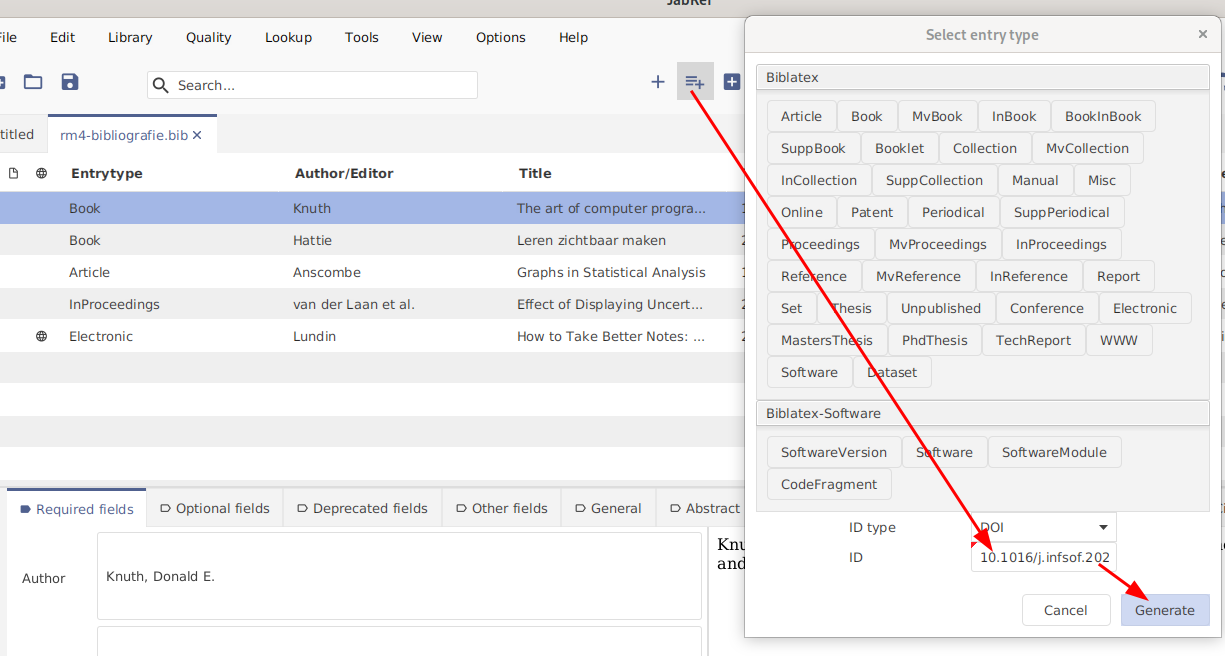
\includegraphics[height=.8\textheight]{4/jabref-new-entry-doi}

\end{frame}

\begin{frame}[plain]
  \frametitle{Bibliografische gegevens in Jabref.}
  \framesubtitle{Extra info voor Electronic (Online, WWW)}

  \begin{description}
    \item[Url] Hyperlink naar de bron
    \item[Urldate] Datum van raadplegen
  \end{description}

  \bigskip

  \textbf{Voorbeeld:}

  \bigskip

  \fullcitebib{Lundin2020}

\end{frame}

\begin{frame}[plain]
  \frametitle{Bibliografische gegevens in Jabref.}
  \framesubtitle{Extra info voor InProceedings}

  \begin{description}
    \item[Booktitle] ``Proceedings of the [naam conferentie]''
    \item[Editor] Redacteur(s) (optioneel)
    \item[Pages] paginanummers (optioneel)
  \end{description}

  \medskip

  \textbf{Voorbeeld:}

  \fullcitebib{vanderLaanEtAl2015}
\end{frame}

\begin{frame}
  \frametitle{Bibliografische gegevens in Jabref.}

  Vul zoveel mogelijk info in (maakt zoeken gemakkelijker):

  \begin{description}
    \item[DOI] Digital Object Identifier: uniek ID voor artikel, hiermee kan je automatisch alle velden invullen
    \item[URL] ook al is het niet echt een Electronic bron
    \item[Keywords] Sleutelwoorden
    \item[File] PDF van de publicatie
    \item[Abstract] Samenvatting
    \item[Comments] Je eigen samenvatting/opmerkingen
  \end{description}

\end{frame}

\section{Refereren naar de literatuur.}

\begin{frame}[fragile]
  \frametitle{Refereren in de tekst}

  \begin{itemize}
    \item \verb|\textcite{Knuth1998}| \(\Rightarrow\) Knuth (1998)
    \item \verb|\autocite{Knuth1998}| \(\Rightarrow\) (Knuth, 1998)
  \end{itemize}

\end{frame}

\begin{frame}
  \frametitle{Gebruik \texttt{\textbackslash{}textcite}}

  \ldots\ als de naam van de auteur onderdeel is van de zin:

  \bigskip

  \begin{quotation}
    An overview is provided in the survey by Ribas et al (2010). For a real-life case-study of applying genetic algorithm ``on top'' of a Mixed Integer Linear Programming model, we refer to Borodin et al (2011).
  \end{quotation}

\end{frame}

\begin{frame}
  \frametitle{Gebruik \texttt{\textbackslash{}autocite}}

  \ldots\ als de naam van de auteur GEEN onderdeel is van de zin:

  \bigskip

  \begin{quotation}
    Reinforcement Learning (RL) is a technique that allows an agent to learn how to maximize a numerical reward signal (Sutton and Barto, 1998).
  \end{quotation}

  \bigskip
  
  Ook: bij letterlijk citaat, bronvermelding afbeelding

\end{frame}


%% TODO: uitgewerkte voorbeelden! \textcite, \autocite, citaat, bijschrift afbeelding?

\begin{frame}[fragile]
  \frametitle{Referentielijst toevoegen.}

  \begin{itemize}
    \item Literatuurlijst invoegen: \verb|\printbibliography|

    \item Compileren (in TexStudio):

    \begin{enumerate}
      \item Build/Compile (F5): bronnen worden nog niet toegevoegd, ``keys'' van bronnen in het vet aangeduid
      \item Bibliography (F8): selecteert de gerefereerde bronnen en maakt ze klaar
      \item Build/Compile (F5): effectief invoegen verwijzingen en literatuurlijst
    \end{enumerate}
  \end{itemize}
\end{frame}

\begin{frame}
  \frametitle{Controleer het resultaat!}

  \begin{itemize}
    \item Auteurs correct weergegeven?
    \item Taal- of zetfouten? Bv.\ accentletters, speciale tekens
    \item Alle info om bron terug te vinden aanwezig?
    \item Vermelding ``Verkregen DATUM, van URL'' bij Online bronnen?
    \item \ldots
  \end{itemize}

\end{frame}

\begin{frame}
  \frametitle{Vaak voorkomende problemen}

  \begin{itemize}
    \item Niet-wetenschappelijke bronnen gebruikt (bv. StackOverflow, Wikipedia, blogs niet van een vakexpert, \ldots)
    \item Niet opgeruimde URLs weergegeven (bv. markers zoals \texttt{\#:$\sim$:text=something} in URL - Scroll To Text Fragment feature van browsers)
    \item Incorrecte of ontbrekende info (bv. ontbrekende paginanummers, verkeerde volgorde van auteurs, verkeerde auteur \ldots)
    \item Foutief type bron (bv. \texttt{Online} in plaats van \texttt{Book} indien het een boek betreft - typisch bij boeken gevonden via Google Books)
    \item \ldots
  \end{itemize}
\end{frame}

\begin{frame}[plain]
  \frametitle{Oefening}

  Sla deze bronnen op in JabRef, met alle nodige info en fulltext (waar mogelijk) en/of URL van de online bron:

  \bigskip

  \begin{itemize}
    \item \url{https://www.sciencedirect.com/science/article/abs/pii/S0020025510002756}
    \item \url{https://catalogus.hogent.be/catalog/hog01:000617334}
    \item \url{https://martinfowler.com/articles/microservices.html}
    \item \url{https://www.youtube.com/watch?v=wW9CAH9nSLs&t=13s}
    \item \url{https://link.springer.com/book/10.1007/978-1-4842-6399-0}
    \item \url{http://www.schedulingconference.org/proceedings/2013/mista2013.pdf} (pp.\ 402--409)
    \item \url{https://docs.ansible.com/ansible-core/devel/index.html}
  \end{itemize}

\end{frame}

\begin{frame}
  \frametitle{Opdracht}

  \begin{itemize}
    \item Sla alle gevonden bronnen op in .bib-bestand
    \item Structureren, bv.\ ahv Mind Map
      \begin{itemize}
        \item Freemind, Gitmind, Xmind, Minder, Vym, \ldots
      \end{itemize}
    \item Verwerk wat je gelezen hebt tot een doorlopende tekst
  \end{itemize}

  \bigskip

  \alertbox{Dit is de belangrijkste fase van de opdracht!}
\end{frame}

\end{document}
